% ==========================================
% CHƯƠNG 3: MÔ HÌNH VÀ HỆ THỐNG ĐỀ XUẤT
% ==========================================
\chapter{MÔ HÌNH VÀ HỆ THỐNG ĐỀ XUẤT}
\label{Chapter3}

% ------------------------------------------------------------
\section{Mô hình phân đoạn PGA-UNet}
\label{sec:pga_unet}
% ------------------------------------------------------------

PGA-UNet (\textit{Prompt-Guided Attention U-Net}) là mô hình phân đoạn tương tác nhận đồng thời ảnh X-quang và hộp giới hạn vùng nghi ngờ. Mô hình này được xây dựng dựa trên khung mã hóa, giải mã của U-Net~\cite{ronneberger2015unet} và ý tưởng chú ý ở kết nối tắt của Attention U-Net~\cite{oktay2018attentionunet}. Từ đó, khóa luận bổ sung ba thành phần chính là bản đồ nhiệt câu nhắc dạng cao nguyên, Cổng không gian tại bộ mã hóa (PSG) và Cơ chế chú ý có điều kiện ở các kết nối tắt của nhánh giải mã (CAD).

Bảng~\ref{tab:inheritance_contribution} phân biệt các thành phần kế thừa với thiết kế được sử dụng trong PGA-UNet.

\begin{table}[htbp]
    \centering
    \caption{Các thành phần kế thừa và thiết kế trong PGA-UNet}
    \label{tab:inheritance_contribution}
    \renewcommand{\arraystretch}{1.3}
    \setlength{\tabcolsep}{4pt}
    \small
    \begin{tabular}{|p{3.1cm}|p{5.1cm}|p{6.1cm}|}
        \hline
        \textbf{Thành phần}
        & \textbf{Cơ sở kế thừa}
        & \textbf{Thiết kế trong PGA-UNet} \\
        \hline
        Khung mạng
        & U-Net~\cite{ronneberger2015unet}: cấu trúc mã hóa, giải mã và kết nối tắt
        & Sử dụng làm kiến trúc nền cho mô hình phân đoạn hạng nhẹ \\
        \hline
        Biểu diễn câu nhắc
        & Các phương pháp phân đoạn có hướng dẫn bằng hộp giới hạn
        & Chuyển hộp giới hạn thành bản đồ nhiệt dạng cao nguyên có biên được làm mềm bằng bộ lọc Gaussian \\
        \hline
        PSG
        & Các phương pháp tích hợp bản đồ không gian vào CNN, chẳng hạn DeepIGeoS~\cite{wang2019deepigeos}
        & Điều biến đặc trưng tại bộ mã hóa bằng cơ chế cổng nhân có kết nối dư \\
        \hline
        CAD
        & Cổng chú ý tại kết nối tắt của Attention U-Net~\cite{oktay2018attentionunet}
        & Điều kiện hóa tín hiệu chú ý tại bộ giải mã bằng đặc trưng câu nhắc \\
        \hline
    \end{tabular}
\end{table}

Hình~\ref{fig:pga_architecture} cho thấy kiến trúc tổng thể của mô hình. Nói ngắn gọn, PSG giúp đưa câu nhắc vào phần trích xuất đặc trưng, còn CAD giữ ảnh hưởng của câu nhắc khi mô hình khôi phục lại mặt nạ. Nhờ vậy, thông tin định vị không chỉ xuất hiện ở đầu vào rồi yếu dần đi, mà còn được dùng lại ở nhiều tầng bên trong mạng.

\begin{figure}[htbp]
    \centering
    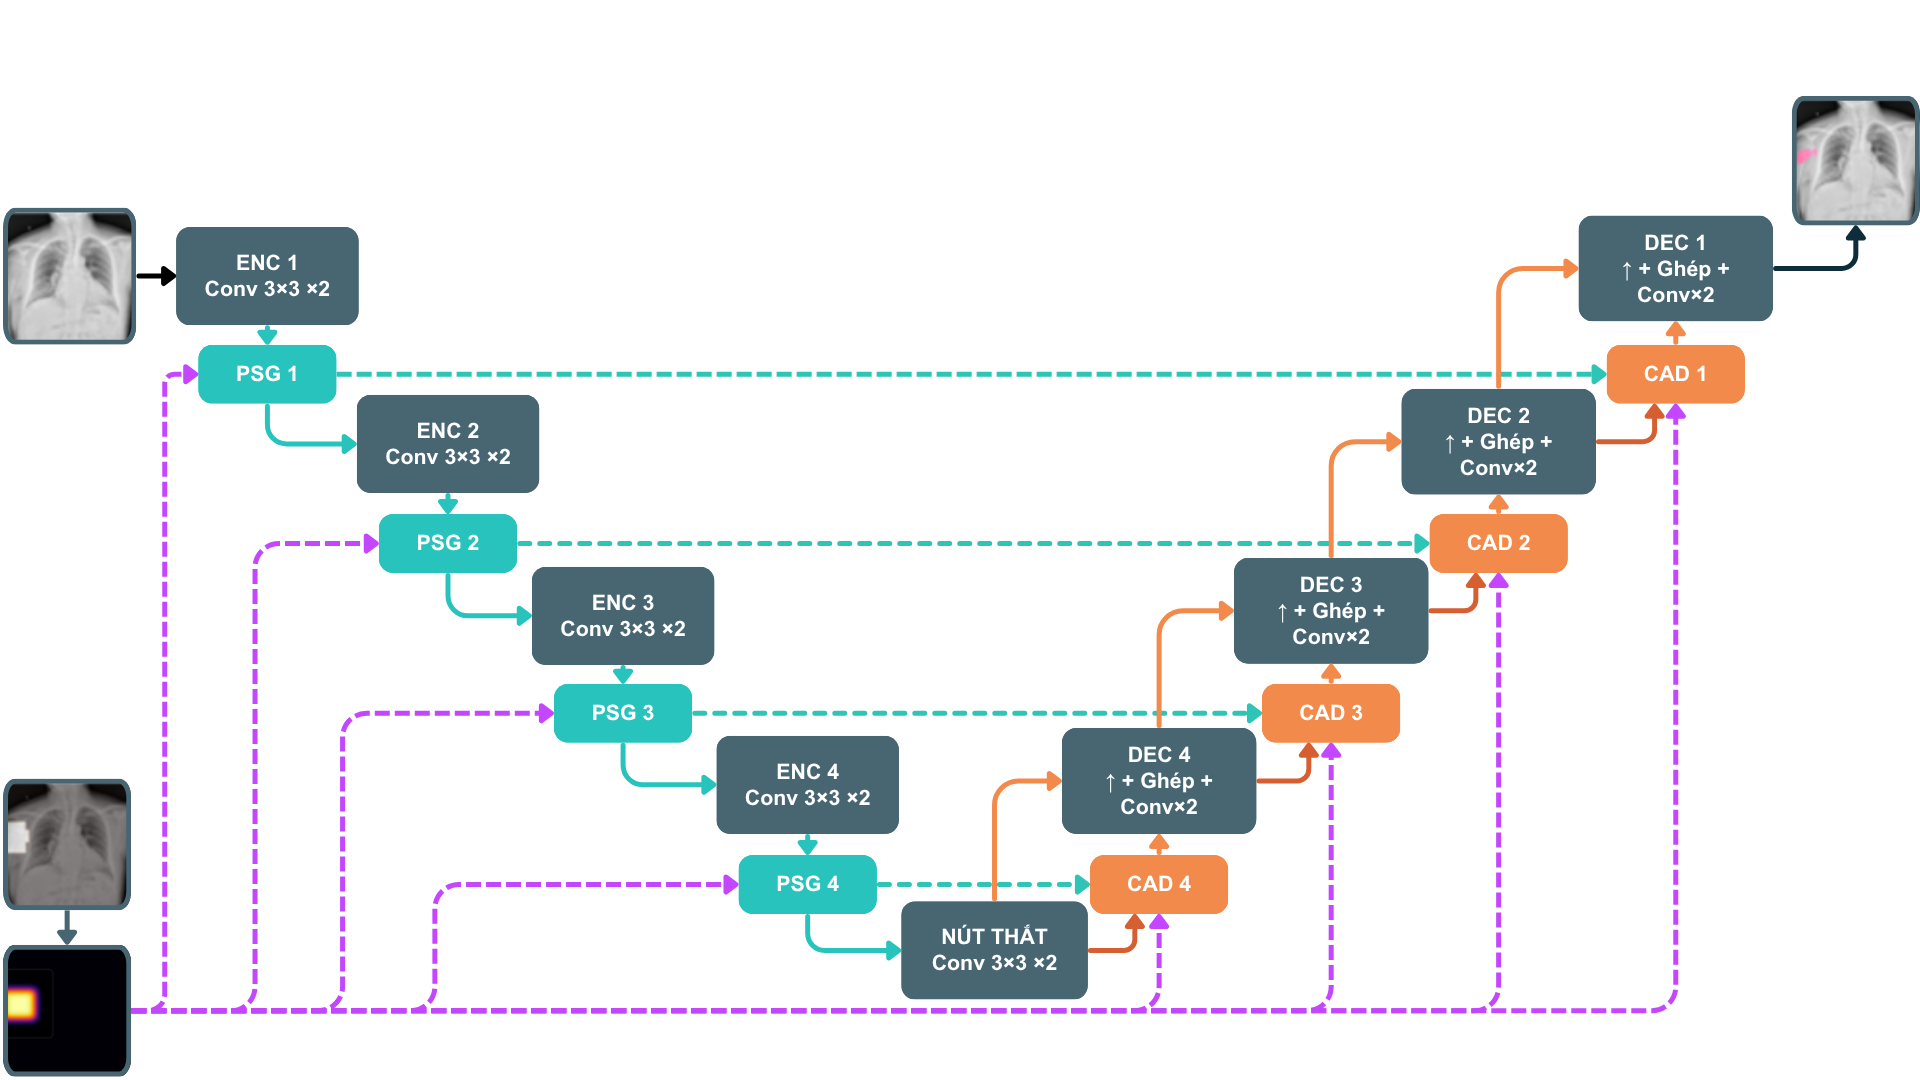
\includegraphics[width=\textwidth]{images/arch_pga_unet2d.png}
    \caption{Kiến trúc PGA-UNet với PSG tại bộ mã hóa và CAD trên các kết nối tắt của nhánh giải mã.}
    \label{fig:pga_architecture}
\end{figure}

% ------------------------------------------------------------
\subsection{Biểu diễn câu nhắc trực quan}
\label{subsec:plateau_heatmap}
% ------------------------------------------------------------

Đầu vào tương tác của PGA-UNet là hộp giới hạn
$\mathbf{B}=(x_1,y_1,x_2,y_2)$ do bác sĩ chẩn đoán ảnh cung cấp quanh vùng nghi ngờ. Các nghiên cứu phân đoạn tương tác khác còn sử dụng điểm nhấp chuột~\cite{xu2016deepinteractive} hoặc nét vẽ tự do~\cite{wang2019deepigeos} làm câu nhắc; khóa luận chọn hộp giới hạn vì đây là thao tác đơn giản, không đòi hỏi bác sĩ ước lượng chính xác tâm hay đường biên tổn thương, đồng thời thống nhất với dạng câu nhắc mà SAM và SAM-Med2D hỗ trợ, thuận lợi cho việc so sánh trực tiếp tại Chương~\ref{Chapter4}. Thay vì sử dụng trực tiếp bốn tọa độ rời rạc, hộp được chuyển thành bản đồ nhiệt câu nhắc
$\mathbf{H}_{\mathrm{prompt}}\in[0,1]^{H\times W}$ có cùng kích thước không gian với ảnh đầu vào.

Trước tiên, hộp giới hạn được biểu diễn thành mặt nạ nhị phân:

\begin{equation}
    \mathbf{B}_{\mathrm{mask}}(x,y)
    =
    \begin{cases}
        1, & (x,y)\in\mathbf{B},\\
        0, & \text{ngược lại}.
    \end{cases}
    \label{eq:bbox_mask}
\end{equation}

Biên của mặt nạ sau đó được làm mềm bằng bộ lọc Gaussian:

\begin{equation}
    \mathbf{H}_{\mathrm{prompt}}
    =
    \mathbf{B}_{\mathrm{mask}}
    \ast
    \mathbf{K}_{\mathrm{Gaussian}}(k),
    \qquad k=31,
    \label{eq:plateau_heatmap}
\end{equation}

trong đó $\ast$ là phép tích chập và
$\mathbf{K}_{\mathrm{Gaussian}}(k)$ là nhân Gaussian có kích thước $k\times k$. Hộp giới hạn được mở rộng thêm 5 điểm ảnh ở mỗi cạnh trước khi tạo mặt nạ nhằm hạn chế việc cắt sát đường biên tổn thương.

Cách biểu diễn này tạo ra một vùng có giá trị cao tương đối đều ở bên trong hộp và mềm hơn ở phần biên. So với mặt nạ nhị phân, tín hiệu này bớt gắt hơn và có thể giúp mô hình đỡ phụ thuộc vào đường biên cứng của hộp. So với một phân phối Gaussian chỉ nhấn vào vùng tâm, dạng cao nguyên vẫn giữ thông tin trên gần như toàn bộ vùng được khoanh.

Bản đồ nhiệt được dùng như một nhánh dữ liệu riêng song song với ảnh X-quang. Vì có cùng cấu trúc không gian $H\times W$ với ảnh, nó có thể được giảm mẫu để phù hợp với nhiều tầng đặc trưng khác nhau trong CNN.

Khác với các mô hình nền tảng như SAM và SAM-Med2D~\cite{2023-SAM-Kirillov,2023-SAMMed2D-Cheng}, nơi hộp giới hạn thường được mã hóa thành biểu diễn nhúng phù hợp với Transformer, PGA-UNet giữ câu nhắc dưới dạng bản đồ hai chiều. Cách làm này hợp với CNN hơn và thuận tiện cho việc điều biến đặc trưng theo từng vị trí không gian.

% ------------------------------------------------------------
\subsection{Cổng không gian tại bộ mã hóa}
\label{subsec:psg}
% ------------------------------------------------------------

Trong U-Net thông thường, bộ mã hóa trích xuất đặc trưng trên toàn bộ ảnh mà không biết bác sĩ đang quan tâm vùng nào. Với ảnh X-quang, điều này có thể làm mô hình bị phân tán bởi nền ảnh, vùng xương chồng lấp hoặc các khu vực có tương phản mạnh nhưng không liên quan trực tiếp đến tổn thương.

Vì vậy, PGA-UNet thêm Cổng không gian PSG (\textit{Prompt Spatial Gate}) vào các tầng mã hóa. Vai trò của PSG là dùng bản đồ nhiệt để điều chỉnh đặc trưng theo không gian, giúp mô hình chú ý sớm hơn đến vùng được khoanh.

Tại tầng mã hóa thứ $l$, bản đồ nhiệt được giảm mẫu bằng nội suy song tuyến tính về cùng độ phân giải với đặc trưng $\mathbf{x}^{l}$:

\begin{equation}
    \mathbf{H}^{l}
    =
    \operatorname{Bilinear}
    \left(
        \mathbf{H}_{\mathrm{prompt}},
        \frac{H}{2^{l}},
        \frac{W}{2^{l}}
    \right).
    \label{eq:psg_downsample}
\end{equation}

Bản đồ sau khi giảm mẫu được đưa qua phép tích chập $1\times1$ và hàm Sigmoid để sinh trọng số điều biến:

\begin{equation}
    \mathbf{A}^{l}_{\mathrm{PSG}}
    =
    \sigma
    \left(
        \mathbf{W}^{l}_{\mathrm{gate}}
        \ast
        \mathbf{H}^{l}
    \right),
    \label{eq:psg_attention}
\end{equation}

trong đó $\mathbf{W}^{l}_{\mathrm{gate}}$ ánh xạ bản đồ một kênh sang cùng số kênh với đặc trưng $\mathbf{x}^{l}$. Đặc trưng đầu ra của PSG được xác định bởi:

\begin{equation}
    \widetilde{\mathbf{x}}^{l}
    =
    \mathbf{x}^{l}
    \odot
    \left(
        1+
        \alpha^{l}_{\mathrm{PSG}}
        \mathbf{A}^{l}_{\mathrm{PSG}}
    \right),
    \label{eq:spatial_gate}
\end{equation}

với $\odot$ là phép nhân theo phần tử và
$\alpha^{l}_{\mathrm{PSG}}\in[0,1]$ là hệ số học được, được khởi tạo bằng 0 hoặc 1.

Thành phần $1+$ trong Phương trình~\eqref{eq:spatial_gate} tạo ra kết nối dư, giúp đặc trưng gốc không bị mất đi. Nói cách khác, PSG trong khóa luận không được thiết kế để triệt hẳn phần nền, mà thiên về việc tăng cường vùng đã được câu nhắc chỉ ra trong khi vẫn giữ lại ngữ cảnh chung của ảnh.

So với cách chỉ ghép câu nhắc ở đầu vào, PSG giúp tín hiệu định hướng đi vào nhiều mức đặc trưng khác nhau của bộ mã hóa. Tác dụng riêng của PSG và tác dụng khi phối hợp với CAD sẽ được kiểm tra ở phần thực nghiệm loại bỏ thành phần trong Chương~\ref{Chapter4}.

% ------------------------------------------------------------
\subsection{Cơ chế chú ý có điều kiện trên kết nối tắt của nhánh giải mã}
\label{subsec:cad}
% ------------------------------------------------------------

PSG giúp đưa câu nhắc vào bộ mã hóa, nhưng khi đặc trưng đi qua nhiều tầng sâu thì ảnh hưởng của tín hiệu định vị vẫn có thể yếu dần. Vì vậy, PGA-UNet tiếp tục bổ sung CAD (\textit{Conditional Attention Decoder}) ở các kết nối tắt của nhánh giải mã để giữ lại ảnh hưởng của câu nhắc trong quá trình khôi phục mặt nạ.

Trong Attention U-Net~\cite{oktay2018attentionunet}, hệ số chú ý tại kết nối tắt được tính từ đặc trưng bộ mã hóa $\mathbf{x}^{l}$ và tín hiệu cổng $\mathbf{g}^{l}$ của bộ giải mã. Tín hiệu này được hình thành hoàn toàn từ đặc trưng nội bộ của mạng và không nhận trực tiếp thông tin từ câu nhắc.

Trong CAD, bản đồ nhiệt được giảm mẫu về cùng độ phân giải với tín hiệu cổng và đưa qua bộ mã hóa câu nhắc:

\begin{equation}
    \mathbf{p}^{l}_{\mathrm{enc}}
    =
    f^{l}_{\mathrm{enc}}
    \left(
        \operatorname{Resize}
        \left(
            \mathbf{H}_{\mathrm{prompt}},
            \operatorname{size}(\mathbf{g}^{l})
        \right)
    \right),
    \label{eq:prompt_encoding}
\end{equation}

trong đó $f^{l}_{\mathrm{enc}}$ gồm hai lớp tích chập $3\times3$ liên tiếp, mỗi lớp theo sau bởi phép chuẩn hóa theo từng mẫu (\textit{Instance Normalization}) và hàm ReLU. Trong triển khai hiện tại, khối này ánh xạ bản đồ một kênh thành biểu diễn có cùng số kênh với tín hiệu cổng tại tầng giải mã thứ $l$: lớp thứ nhất tạo số kênh bằng một nửa số kênh của tín hiệu cổng, lớp thứ hai nâng lên đúng số kênh của tín hiệu cổng.

Từ biểu diễn này, một hệ số điều chế câu nhắc được xác định:

\begin{equation}
    c^{l}
    =
    \sigma
    \left(
        \operatorname{GAP}
        \left(
            \mathbf{p}^{l}_{\mathrm{enc}}
        \right)
    \right),
    \label{eq:prompt_confidence}
\end{equation}

trong đó $\operatorname{GAP}$ là phép gộp trung bình toàn cục. Trong triển khai, $c^{l}$ là một hệ số vô hướng theo từng mẫu (dạng bản đồ $1\times1\times1$ sau phép tích chập $1\times1$ và hàm Sigmoid), dùng để điều chỉnh mức ảnh hưởng tổng thể của đặc trưng câu nhắc tại tầng tương ứng; nó không được diễn giải là xác suất tin cậy đã hiệu chỉnh.

Tín hiệu cổng được điều kiện hóa bởi đặc trưng câu nhắc:

\begin{equation}
    \mathbf{g}'^{\,l}
    =
    \mathbf{g}^{l}
    +
    c^{l}
    \alpha^{l}_{\mathrm{CAD}}
    w_l
    \mathbf{p}^{l}_{\mathrm{enc}},
    \label{eq:conditioned_gate}
\end{equation}

trong đó $\alpha^{l}_{\mathrm{CAD}}$ là hệ số pha trộn học được và $w_l$ điều chỉnh mức ảnh hưởng của câu nhắc tại từng tầng giải mã. Trong mã nguồn thực nghiệm, mỗi tầng giải mã có một tham số vô hướng riêng $\alpha^{l}_{\mathrm{CAD}}=\sigma(\alpha^{l}_{\mathrm{raw}})$ và bộ trọng số cố định $w_l=\{1{,}0;\,0{,}7;\,0{,}4;\,0{,}2\}$ theo thứ tự từ tầng sâu đến tầng nông.

Hệ số chú ý tại kết nối tắt được tính bởi:

\begin{equation}
    \mathbf{A}^{l}_{\mathrm{CAD}}
    =
    \sigma
    \left[
        \boldsymbol{\psi}^{l}
        \ast
        \delta
        \left(
            \mathbf{W}^{l}_{x}\ast\widetilde{\mathbf{x}}^{l}
            +
            \mathbf{W}^{l}_{g}\ast\mathbf{g}'^{\,l}
        \right)
    \right],
    \label{eq:cad_attention}
\end{equation}

trong đó $\delta$ là hàm ReLU,
$\mathbf{W}^{l}_{x}$ và $\mathbf{W}^{l}_{g}$ là các phép chiếu đặc trưng, còn $\boldsymbol{\psi}^{l}$ ánh xạ kết quả về bản đồ chú ý một kênh. Đặc trưng kết nối tắt sau chú ý được xác định bởi:

\begin{equation}
    \widehat{\mathbf{x}}^{l}
    =
    \widetilde{\mathbf{x}}^{l}
    \odot
    \mathbf{A}^{l}_{\mathrm{CAD}}.
    \label{eq:cad_skip}
\end{equation}

Điểm khác chính của CAD so với cổng chú ý nguyên bản là tín hiệu điều khiển ở đây được điều kiện hóa trực tiếp bởi câu nhắc từ bên ngoài. Có thể xem PSG là phần dẫn hướng ở bước mã hóa, còn CAD là phần nhắc lại định hướng đó ở bước giải mã. Hai thành phần này đi cùng nhau để câu nhắc có ảnh hưởng xuyên suốt mạng, thay vì chỉ xuất hiện ở một chỗ.

\paragraph{Chi tiết triển khai theo tầng.}
Với hệ số thu gọn \texttt{feature\_scale}=4, PGA-UNet sử dụng số kênh $\{16,32,64,128,256\}$ từ tầng mã hóa nông nhất đến nút cổ chai. Bốn tầng giải mã lần lượt nhận cặp kênh bỏ qua/tín hiệu cổng là $(128,256)$, $(64,128)$, $(32,64)$ và $(16,32)$. Ở mỗi tầng giải mã, $f^{l}_{\mathrm{enc}}$ mã hóa prompt theo số kênh của tầng đó, trong đó $g_l$ là tín hiệu từ nút thắt đi lên nên buộc phải giảm số kênh bằng với đặc trưng từ bộ mã hóa (tín hiệu từ nút thắt $g_l \rightarrow g_l/2 \rightarrow g_l$ mới này là tín hiệu của tầng này). Cấu hình này được dùng thống nhất trong toàn bộ thực nghiệm của khóa luận.

Các hệ số $w_l$, tham số khởi tạo và các thiết lập thực nghiệm được sử dụng thống nhất trong các phép đánh giá của khóa luận. Giá trị cụ thể được trình bày tại Chương~\ref{Chapter4}.

% ------------------------------------------------------------
\section{Quy trình huấn luyện và suy luận}
\label{sec:algorithm_summary}
% ------------------------------------------------------------

Phần này tóm tắt hai quy trình chính của PGA-UNet là huấn luyện và suy luận. Khi huấn luyện, hộp giới hạn được tạo từ mặt nạ nhãn gốc rồi điều chỉnh để mô phỏng sai lệch thao tác. Khi suy luận, mô hình nhận trực tiếp hộp giới hạn từ bác sĩ chẩn đoán ảnh.

% ------------------------------------------------------------
\subsection{Quy trình huấn luyện}
\label{subsec:training_process}
% ------------------------------------------------------------

Đầu vào huấn luyện gồm ảnh X-quang và mặt nạ phân đoạn. Với mỗi mẫu, hộp giới hạn được trích từ mặt nạ, sau đó biến đổi theo kịch bản câu nhắc Bao trọn hoặc Lệch tâm. Trong mô phỏng câu nhắc, gọi $w=x_2-x_1$ và $h=y_2-y_1$ lần lượt là chiều rộng và chiều cao
của hộp bao sát tổn thương. Ba kịch bản câu nhắc được xây dựng như sau:

\begin{itemize}
    \item \textbf{Bao trọn:} Hộp bao sát được mở rộng với tỷ lệ
    $r\in[0{,}15;0{,}45]$ theo kích thước ban đầu, nhằm mô phỏng thao
    tác khoanh rộng hơn vùng tổn thương.

    \item \textbf{Lệch tâm:} Hộp được dịch khỏi vị trí ban đầu theo
    hướng ngẫu nhiên với hệ số dịch bằng $0{,}30$ kích thước hộp. Tọa độ sau biến đổi được giới hạn trong
    phạm vi ảnh.

    \item \textbf{Hỗn hợp:} Mỗi mẫu sử dụng câu nhắc Bao trọn với xác
    suất 70\% hoặc câu nhắc Lệch tâm với xác suất 30\%.
\end{itemize}

Các phép biến đổi này chỉ tác động lên hộp giới hạn, còn ảnh X-quang và mặt nạ nhãn gốc vẫn được giữ nguyên. Thiết lập này được áp dụng thống nhất trong các thí nghiệm của PGA-UNet. Từ hộp giới hạn, bản đồ nhiệt câu nhắc được tạo ra và đưa cùng với ảnh vào mô hình. Hàm mất mát dùng để tối ưu là tổ hợp Binary Cross-Entropy và Dice Loss.

\begin{algorithm}[H]
\caption{Quy trình huấn luyện PGA-UNet}
\label{alg:offline}
\begin{algorithmic}[1]
\Require Tập dữ liệu
$\mathcal{D}
=
\{(\mathbf{I}_i,\mathbf{M}_i)\}_{i=1}^{N}$
\Ensure Bộ tham số đã huấn luyện $\boldsymbol{\theta}^{*}$

\State Khởi tạo tham số PGA-UNet $\boldsymbol{\theta}$
\While{chưa thỏa tiêu chí dừng trên tập xác thực}
    \For{mỗi lô nhỏ $(\mathbf{I},\mathbf{M})$}
        \State Chuẩn hóa ảnh và mặt nạ theo cùng hệ số
        \State Trích hộp giới hạn $\mathbf{B}$ từ mặt nạ $\mathbf{M}$
        \State Điều chỉnh $\mathbf{B}$ theo kịch bản câu nhắc được chọn
        \State Tạo bản đồ nhiệt
        $\mathbf{H}_{\mathrm{prompt}}$
        từ $\mathbf{B}$
        \State Dự đoán
        $\widehat{\mathbf{Y}}
        \leftarrow
        f_{\mathrm{PGA}}
        (\mathbf{I},\mathbf{H}_{\mathrm{prompt}};\boldsymbol{\theta})$
        \State Tính
        $\mathcal{L}
        \leftarrow
        \mathcal{L}_{\mathrm{BCE}}
        +
        \mathcal{L}_{\mathrm{Dice}}$
        \State Cập nhật $\boldsymbol{\theta}$ bằng bộ tối ưu AdamW
    \EndFor
    \State Đánh giá mô hình trên tập xác thực
    \If{thỏa tiêu chí dừng trên tập xác thực}
        \State Kết thúc vòng lặp huấn luyện
    \EndIf
\EndWhile
\State \Return
$\boldsymbol{\theta}^{*}
\leftarrow$
tham số của mô hình được chọn cho đánh giá
\end{algorithmic}
\end{algorithm}

Mô hình được huấn luyện riêng trên từng bộ dữ liệu. Các cấu hình cụ thể hơn sẽ được nêu ở Chương~\ref{Chapter4}.

% ------------------------------------------------------------
\subsection{Quy trình suy luận}
% ------------------------------------------------------------

Trong giai đoạn suy luận, bác sĩ cung cấp ảnh X-quang và hộp giới hạn vùng nghi ngờ. Hộp được chuyển thành bản đồ nhiệt theo cùng phương pháp sử dụng khi huấn luyện. Mô hình trả về bản đồ xác suất, sau đó được nhị phân hóa tại ngưỡng 0,5 để tạo mặt nạ cuối cùng.

\begin{algorithm}[H]
\caption{Quy trình suy luận PGA-UNet}
\label{alg:online}
\begin{algorithmic}[1]
\Require Ảnh X-quang $\mathbf{I}$ và hộp giới hạn
$\mathbf{B}=(x_1,y_1,x_2,y_2)$
\Ensure Mặt nạ phân đoạn $\widehat{\mathbf{M}}$

\If{$\mathbf{B}=\emptyset$}
    \State \Return thông báo yêu cầu cung cấp hộp giới hạn
\EndIf
\State Chuẩn hóa ảnh $\mathbf{I}$ để phù hợp với kích thước đầu vào
\State Tạo mặt nạ hộp giới hạn $\mathbf{B}_{\mathrm{mask}}$
\State Tạo bản đồ nhiệt
$\mathbf{H}_{\mathrm{prompt}}
\leftarrow
\mathbf{B}_{\mathrm{mask}}
\ast
\mathbf{K}_{\mathrm{Gaussian}}(31)$
\State Tính xác suất phân đoạn
$\widehat{\mathbf{Y}}
\leftarrow
f_{\mathrm{PGA}}
(\mathbf{I},\mathbf{H}_{\mathrm{prompt}};\boldsymbol{\theta}^{*})$
\State Tạo mặt nạ
$\widehat{\mathbf{M}}
\leftarrow
\mathbf{1}[\widehat{\mathbf{Y}}\geq0{,}5]$
\State \Return $\widehat{\mathbf{M}}$
\end{algorithmic}
\end{algorithm}

Nếu bác sĩ chưa cung cấp hộp giới hạn thì hệ thống sẽ không phân đoạn. Lý do là bản đồ nhiệt toàn giá trị 0 không mang thông tin định vị, nên không đúng với cách PGA-UNet được thiết kế và huấn luyện.

Quy trình suy luận chỉ cần một lượt truyền xuôi qua mô hình. Với kiến trúc CNN và số kênh cố định, chi phí tính toán của PGA-UNet tăng theo kích thước ảnh đầu vào. Theo thống kê kiến trúc, mô hình có khoảng 3 triệu tham số. Trong khóa luận, số lượng tham số, FLOPs, bộ nhớ đỉnh, độ trễ suy luận và dung lượng checkpoint của PGA-UNet và SAM-Med2D cũng được đo trong cùng môi trường thực nghiệm; kết quả được trình bày ở Mục~\ref{subsec:efficiency_measurement}, Chương~\ref{Chapter4}. Các con số này chỉ nên hiểu là so sánh tương đối trong cùng môi trường đo.

% ------------------------------------------------------------
\section{Mở rộng luồng xử lý với mô-đun sàng lọc}
\label{sec:tong_the}
% ------------------------------------------------------------

PGA-UNet được huấn luyện cho trường hợp ảnh đã có vùng nghi ngờ và bác sĩ đã cung cấp hộp giới hạn. Trong thực tế, luồng ảnh đầu vào có thể lẫn cả ảnh bình thường và ảnh bệnh lý. Vì vậy, để minh họa cách PGA-UNet có thể đặt trong một quy trình lớn hơn, khóa luận bổ sung Gatekeeper dùng EfficientNet-B3 trước bước phân đoạn.

Gatekeeper chỉ là phần hỗ trợ thêm, không phải đóng góp kiến trúc chính của khóa luận. Mô-đun này trả về xác suất bất thường để bác sĩ tham khảo, chứ không tự động loại bỏ ảnh hay thay cho quyết định của bác sĩ chẩn đoán ảnh.

% ------------------------------------------------------------
\subsection{Sàng lọc ảnh đầu vào}
\label{sec:phan_lop}
% ------------------------------------------------------------

Gatekeeper phân loại ảnh thành bình thường hoặc nghi ngờ có bất thường. Với ảnh được gợi ý có bất thường, bác sĩ kiểm tra và cung cấp hộp giới hạn để chuyển sang PGA-UNet. Với ảnh được gợi ý bình thường, bác sĩ vẫn có thể xác nhận lại hoặc chủ động khoanh vùng nếu phát hiện dấu hiệu nghi ngờ.

Cơ chế này được thiết kế theo hướng sàng lọc mềm, tức là Gatekeeper chỉ gợi ý ảnh nào đáng chú ý hơn, còn việc có chuyển sang bước phân đoạn hay không vẫn do bác sĩ chẩn đoán ảnh quyết định. Cách làm này giúp hạn chế rủi ro ảnh bệnh lý bị bỏ qua hoàn toàn chỉ vì mô-đun phân loại đoán sai.

Cấu hình và kết quả thực nghiệm của Gatekeeper trên BTXRD và FracAtlas được tóm tắt tại Mục~\ref{sec:product_overview}, Chương~\ref{Chapter4}, với số liệu chi tiết tại Phụ lục~\ref{AppendixB}.

% ------------------------------------------------------------
\subsection{Phân đoạn có hướng dẫn}
\label{subsec:pga_stage}
% ------------------------------------------------------------

Sau khi xác định vùng nghi ngờ, bác sĩ vẽ hộp giới hạn trên ảnh X-quang. Hệ thống chuyển hộp thành bản đồ nhiệt và đưa đồng thời ảnh với bản đồ câu nhắc vào PGA-UNet. Mặt nạ dự đoán được hiển thị chồng lên ảnh gốc để hỗ trợ quan sát.

Nếu kết quả chưa phù hợp, bác sĩ có thể điều chỉnh hộp giới hạn và thực hiện lại suy luận. Quá trình hiệu chỉnh chỉ thay đổi câu nhắc đầu vào, không cập nhật kiến trúc hoặc tham số mô hình.

\begin{figure}[H]
    \centering
    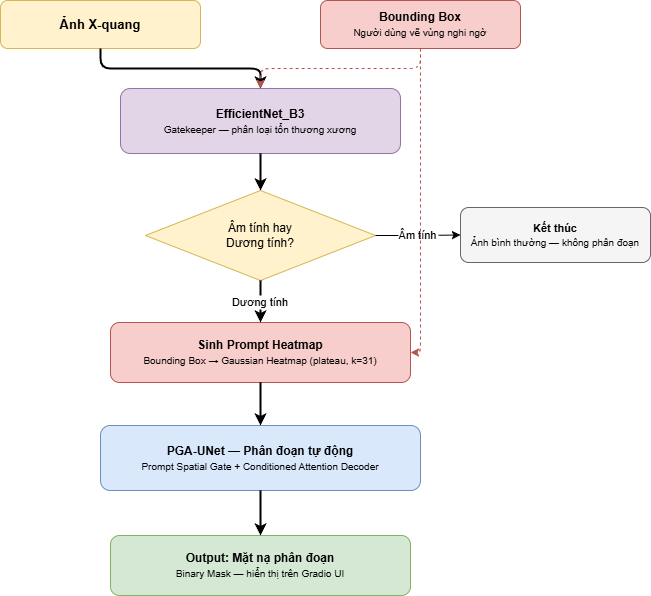
\includegraphics[
        width=0.88\textwidth,
        keepaspectratio
    ]{images/pipeline_pga_app_inference.png}
    \caption{Luồng xử lý hỗ trợ gồm Gatekeeper và PGA-UNet.}
    \label{fig:pipeline_overview}
\end{figure}

Luồng trên chỉ nhằm minh họa một cách tích hợp PGA-UNet vào quy trình xử lý ảnh hỗn hợp. Vì khóa luận chưa có thử nghiệm với bác sĩ chuyên môn trong điều kiện thực tế, nên đây chưa thể xem là một quy trình lâm sàng đã được xác nhận.

% ------------------------------------------------------------
\section{Tổng kết chương}
\label{sec:summary_ch3}
% ------------------------------------------------------------

Chương này đã trình bày mô hình PGA-UNet với ba phần chính là bản đồ nhiệt câu nhắc dạng cao nguyên, PSG ở bộ mã hóa và CAD ở các kết nối tắt của nhánh giải mã. PSG giúp đưa thông tin không gian của câu nhắc vào phần trích xuất đặc trưng, còn CAD giúp duy trì ảnh hưởng đó trong lúc mô hình khôi phục mặt nạ.

Ngoài kiến trúc mô hình, chương này cũng mô tả quy trình huấn luyện, suy luận và phần mở rộng với Gatekeeper trong một luồng xử lý hỗ trợ. Hiệu quả của các thành phần này sẽ được kiểm tra bằng thực nghiệm trên BTXRD và FracAtlas ở Chương~\ref{Chapter4}.
